\documentclass{article}

\usepackage{tikzlings}

\begin{document}
	

\begin{tikzpicture}
	\bear
%	\thing[tophat=gray!60!black]
\end{tikzpicture}	

\begin{tikzpicture}
	\penguin
%	\thing[tophat=gray!60!black]
\end{tikzpicture}	

\begin{tikzpicture}
	\marmot
%	\thing[tophat=gray!60!black]
\end{tikzpicture}	

\begin{tikzpicture}
	\koala
%	\thing[tophat=gray!60!black]
\end{tikzpicture}	

\begin{tikzpicture}
	\owl
%	\thing[tophat=gray!60!black]
\end{tikzpicture}	

\begin{tikzpicture}
	\coati
%	\thing[tophat=gray!60!black]
\end{tikzpicture}	

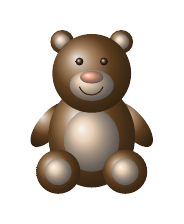
\begin{tikzpicture}
	\bear[3D]
\end{tikzpicture}	

\begin{tikzpicture}
	\penguin[3D]
\end{tikzpicture}	

\begin{tikzpicture}
	\marmot[3D]
\end{tikzpicture}	

\begin{tikzpicture}
	\koala[3D]
\end{tikzpicture}	
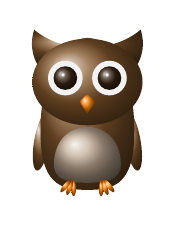
\begin{tikzpicture}
	\owl[3D]
\end{tikzpicture}	

\begin{tikzpicture}
	\coati[3D]
\end{tikzpicture}	


\end{document}
